\documentclass[a4paper,12pt]{article}
\usepackage{geometry} %设置边距,符合Word设定
\geometry{a4paper, top=2.5cm, bottom=2.5cm, left=2.5cm, right=2.5cm}
\usepackage{amsmath} %数学公式排版
\usepackage{lmodern} %使用Latin Modern字体
\usepackage{graphicx} % 引入graphicx包以插入图片
\usepackage{multirow} %单元格合并
\usepackage{makecell} %优化单元格显示
\usepackage{tabularx} %Latex的表格
\usepackage{xeCJK} %排版中日韩(CJK)文字
\usepackage{fontspec} %提供了一个自动和统一的接口来加载字体,\setmainfont用于设置主字体
\usepackage{ctex} %中文支持
\usepackage{cite} %文献引用
\usepackage{extarrows} %更加强大的箭头绘制功能

\setmainfont{Times New Roman}

% 导言区
\title{\heiti\zihao{2} 实验:硫酸亚铁铵的制备}
\author{专业名称\quad 姓\;名\quad 学号xxxxxxxxxxxxxx}
\date{20xx年xx月xx日}

%设置小四号字号,字号为12pt,行距为18pt
\renewcommand{\normalsize}{\fontsize{12pt}{18pt}\selectfont}
%文件开始
\begin{document}

\maketitle

\setcounter{section}{0}
\section*{一、实验原理与操作方法}
\subsection*{(一)实验原理}
六水合硫酸亚铁铵($\rm FeSO_4\cdot (NH_4)_2SO_4\cdot 6H_2O$),俗称“摩尔盐”,是一种浅蓝色的复盐,相较于绿矾($\rm FeSO_4\cdot 7H_2O$)更为稳定,
由于其溶解度小于$\rm FeSO_4\cdot 7H_2O$和$\rm (NH_4)_2SO_4$,使它能从$\rm FeSO_4\cdot 7H_2O$和$\rm (NH_4)_2SO_4$的混合溶液中析出,
制备$\rm FeSO_4\cdot (NH_4)_2SO_4\cdot 6H_2O$的反应式如下:
$$
\rm Fe+H_2SO_4\xlongequal{\quad} FeSO_4+H_2\uparrow
$$$$
\rm FeSO_4+(NH_4)_2SO_4+6H_2O \xlongequal{\quad} FeSO_4\cdot (NH_4)_2SO_4\cdot 6H_2O
$$

由于实验中所涉及到的三种盐类的溶解度均是随温度的降低而降低,且目标产物的溶解度最小,
所以将$\rm FeSO_4\cdot 7H_2O$和$\rm (NH_4)_2SO_4$的混合溶液在较高温度下浓缩,开始结晶之后降温冷却就可以使其析出$\rm FeSO_4\cdot (NH_4)_2SO_4\cdot 6H_2O$晶体。
在过滤时使用乙醇清洗,可以洗去杂质,纯化目标产物

二价铁($\rm Fe^{2+}$)被氧化之后会生成$\rm Fe^{3+}$,它可以与KSCN作用,生成红色配合物,利用这个原理,实验可以采用目视比色法来判断产物中$\rm Fe^{3+}$的含量。

\subsection*{(二)操作方法}

(1)取2g纯铁粉,置于锥形瓶中,另取$\rm 15mL 3mol\cdot L^{-1}$的$\rm H_2SO_4$溶液,加入锥形瓶,在电热板上加热至完全反应,完全反应时溶液中无气泡出现,该步骤可以制得蓝绿色的$\rm FeSO_4$溶液;

(2)加水,稀释至溶液体积达到25mL(锥形瓶上应当提前做好记号),然后趁热过滤,得到澄清滤液;

(3)称量$\rm 4.50g (NH_4)_2SO_4$,加入滤液中,加热搅拌至完全溶解,制得$\rm FeSO_4\cdot 7H_2O$和$\rm (NH_4)_2SO_4$的混合溶液;

(4)混合溶液转入蒸发皿,然后在水浴锅中加热蒸发,直至溶液表面出现固体薄膜,然后取出蒸发皿,使其自然冷却,产生更多的晶体;

(5)进行减压抽滤,并使用少量乙醇冲洗固体,将晶体转移至玻璃表面皿上晾干,而后进行称重、拍照、装袋;

(6)取1g自制产品置于25mL比色管中,加入15mL除氧(加热煮沸可以除氧,应提前准备)的去离子水溶解;

(7)加入$\rm 1.00mL 6mol\cdot L^{-1}$的HCl溶液和$\rm 1.00mL 1mol\cdot L^{-1}$的KSCN溶液,加注去离子水至刻度线,摇匀,将比色管与标准色阶比较,确定产品到达的试剂级别。

\subsection*{(三)产量与产率的计算}
(1)理论产量

查表可以得到以下数据:

\medskip
\begin{tabularx}{13cm}{|p{3.5cm}p{3cm}|p{3.5cm}p{3cm}|}
    \cline{1-4}
    \makecell{化合物或单质} & \makecell{$\rm M/(g\cdot mol^{-1})$} & \makecell{化合物或单质} & \makecell{$\rm M/(g\cdot mol^{-1})$}\\
    \cline{1-4}
    \multicolumn{1}{|c}{$\rm Fe$} &  \multicolumn{1}{c}{55.845} & \multicolumn{1}{|c}{$\rm H_2SO_4$} & \multicolumn{1}{c|}{98.07}\\
    \cline{1-4}
    \multicolumn{1}{|c}{$\rm FeSO_4\cdot (NH_4)_2SO_4\cdot 6H_2O$} &  \multicolumn{1}{c}{392.13} & \multicolumn{1}{|c}{$\rm (NH_4)_2SO_4$} & \multicolumn{1}{c|}{132.13}\\
    \cline{1-4}
\end{tabularx}
\medskip

那么,可以计算得出实验中所用物品的物质的量:
$$
\rm Fe:0.036mol;\quad  H_2SO_4:0.045mol;\quad (NH_4)_2SO_4:0.0341mol
$$

所以,理论产量m应当使用$\rm (NH_4)_2SO_4$计算,理论产量m为:
$$
\rm m=n_{(NH_4)_2SO_4}\times M_{FeSO_4\cdot (NH_4)_2SO_4\cdot 6H_2O}=
\frac{m_{(NH_4)_2SO_4}\times M_{FeSO_4\cdot (NH_4)_2SO_4\cdot 6H_2O}}{M_{(NH_4)_2SO_4}}
$$

(2)实际产量

将自制的产品放在分析天平上称量,可以得到实际产量$\rm m'$。

(3)产率

产率$\eta$采用如下方式计算:
$$
\eta = \frac{m'}{m}\times 100\%
$$

\subsection*{(四)化学反应方程式}
$$
\rm Fe+H_2SO_4\xlongequal{\quad} FeSO_4+H_2\uparrow
$$$$
\rm FeSO_4+(NH_4)_2SO_4+6H_2O \xlongequal{\quad} FeSO_4\cdot (NH_4)_2SO_4\cdot 6H_2O
$$$$
\rm Fe^{3+}+nSCN^-\xlongequal{\quad} [Fe(SCN)_n]^{3-n}
$$

\section*{二、结果与讨论}

由前述公式,计算得到理论产量m为:$\rm m=\frac{4.50\times 392.13}{132.13}g=13.4g$

实验中,测量自制产品的质量,得到实际产量$\rm m'$为12.15g(见下图)。

\medskip
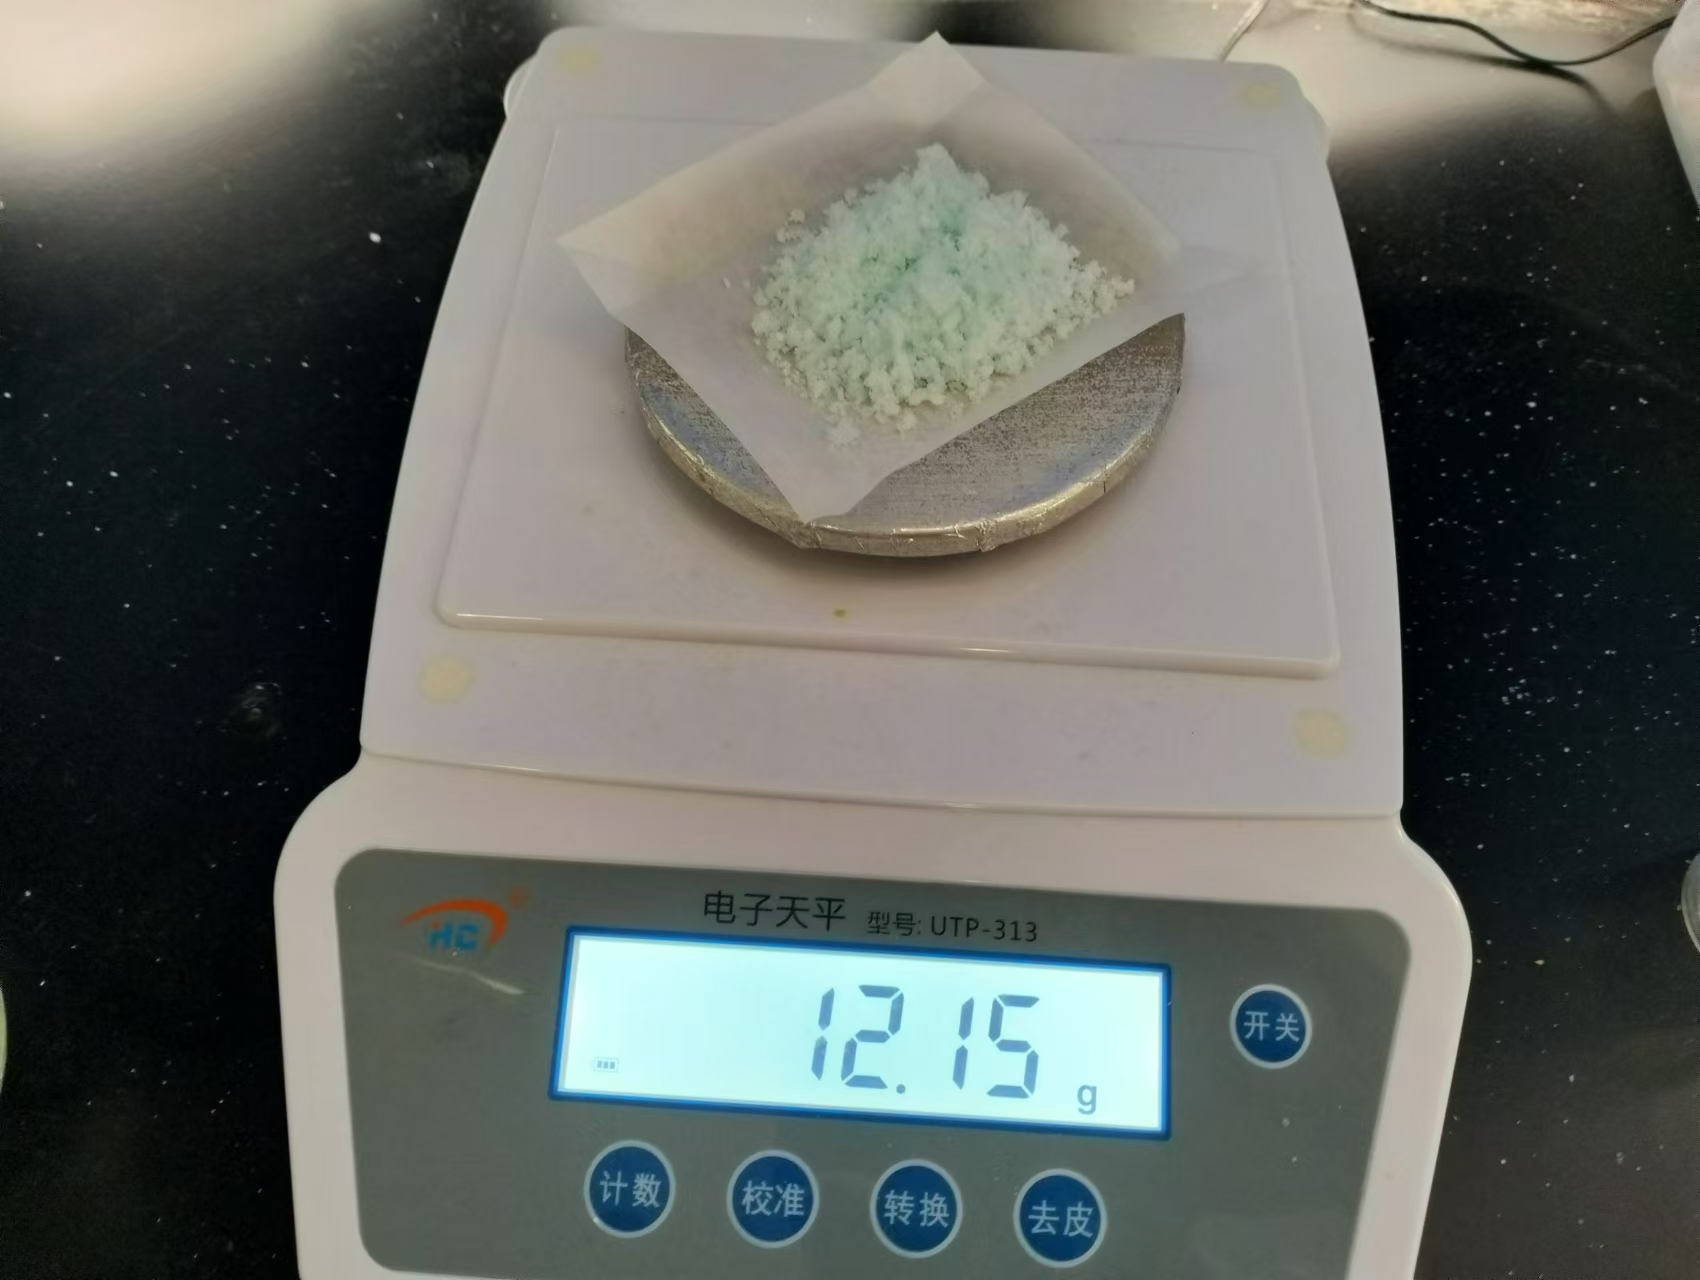
\includegraphics[width=0.5\textwidth]{weight}

因此,得到的产率$\eta$为:
$$
\eta = \frac{m'}{m}\times 100\%=\frac{12.15}{13.4}\times 100\%=90.7\%
$$

采用目视比色法,比较结果如下图:

\medskip
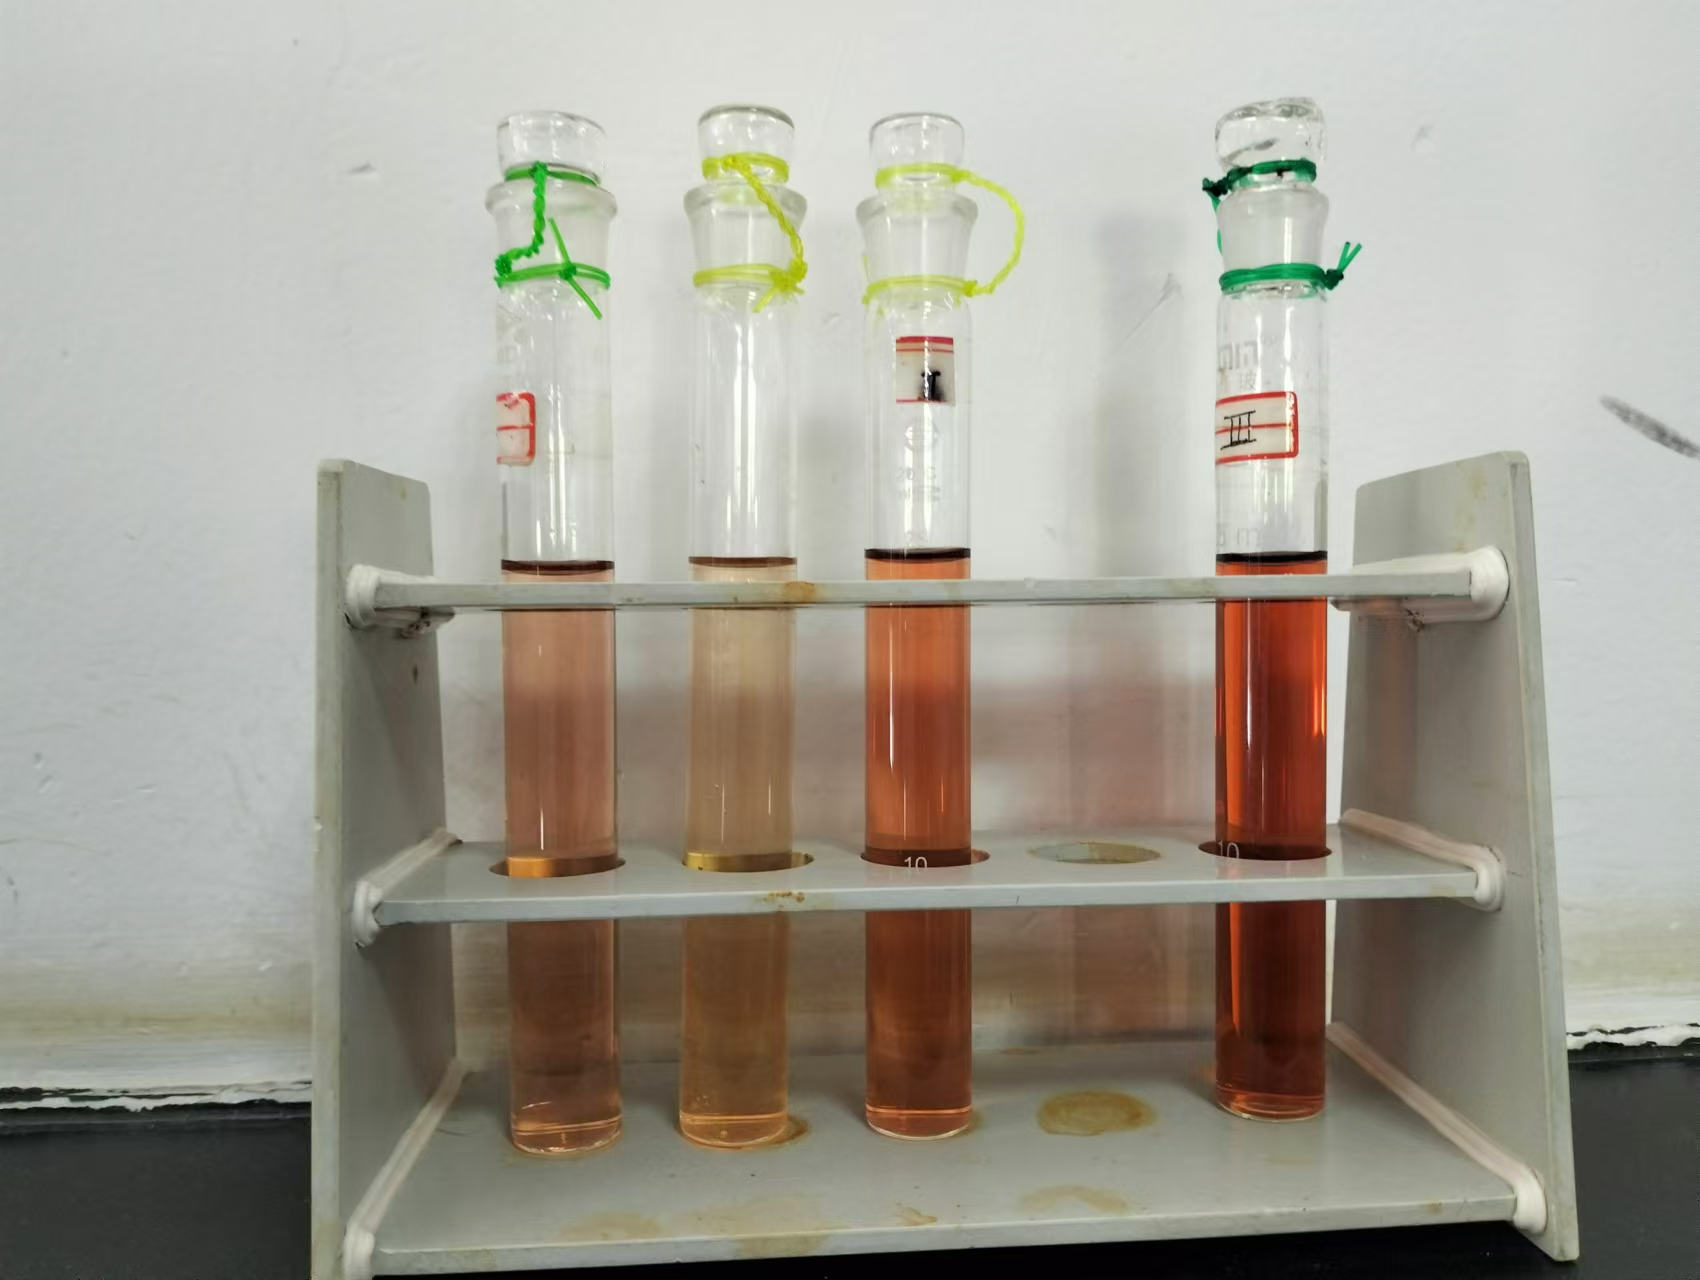
\includegraphics[width=0.5\textwidth]{color}

由此可见,自制的产品中,$\rm Fe^{3+}$的含量较低,产品质量优于I级。

\section*{三、实验分析与总结}
\subsection*{(一)、实验分析}

查阅相关文献\textsuperscript{\cite{GZHA202401061}},并且和同学进行交流,本实验的产品产率偏高,但仍在正常范围内。结合实验中的实际操作,原因可能为:

(1)做实验时,称量的$\rm (NH_4)_2SO_4$质量大于4.50g,导致产率偏大;

(2)由于没有冷却完全,对晶体抽滤时,滤液中形成晶体,实验时重新进行抽滤,从而回收了一部分晶体,使得产率相较于同学的数据偏大;

(3)晶体未完全晾干,使得称重的时候质量偏大;

另,产品中的$\rm Fe^{3+}$含量较低,可能是因为实验操作比较迅速,使得被空气氧化的$\rm Fe^{2+}$较少。

\subsection*{(二)、实验改进}

关于产率略高,可以有以下改进:

(1)严格称量原料的质量与体积,防止$\rm (NH_4)_2SO_4$的质量偏大;

(2)采用冰水进行降温,保证完全冷却,且在冷却完全之后才开始抽滤;

(3)加大乙醇用量,便于冲洗杂质和晾干;

关于提升产率,参考相关文献,可以有以下改进:

(1)不直接加入$\rm (NH_4)_2SO_4$固体,而是加入$\rm (NH_4)_2SO_4$饱和溶液\textsuperscript{\cite{GZHA202401061}},可以使得制备出的晶体质量大,产率高;

(2)生成硫酸亚铁后使用吸铁石吸附去除剩余铁粉,不需要减压抽滤\textsuperscript{\cite{GLKX202311020}},有效减少硫酸亚铁的损失与氧化;

(3)硫酸亚铁合成过程中加入 0.5 mL 浓度为 0.05 mol/L 硫酸铜催化剂\textsuperscript{\cite{GLKX202311020}},构成原电池反应,加快铁的溶解;

(4)硫酸亚铁铵合成时,反应温度控制于$75^{\circ} C$\textsuperscript{\cite{GLKX202311020}},温度过高会使得$\rm Fe^{2+}$容易被氧化,温度较低时会使得反应不充分,该温度下,产品收率最高。

\section*{四、思考题}

(1)制备硫酸亚铁铵时,在蒸发、浓缩过程中,若发现溶液变黄,是什么原因?应如何处理?

若发现溶液变黄,这是因为操作不当导致$\rm Fe^{2+}$被氧化为$\rm Fe^{3+}$,使得溶液显示出$\rm Fe^{3+}$的颜色,即黄色;
此时应当重做实验,并在新一次实验中严格按步骤操作,避免氧化,或者加入还原剂,比如维生素C等,再或者加入过量铁粉,将$\rm Fe^{3+}$还原为$\rm Fe^{2+}$。

(2)干燥硫酸亚铁铵晶体时应注意哪些问题?

干燥晶体时,需要保证通风,并将晶体平摊,增大表面积,便于水分和乙醇的挥发。

(3)以$\rm Na_2C_2O_4$为基准物标定$\rm KMnO_4$溶液的浓度时应注意哪些反应条件?

需要注意“三度”即温度、酸度、滴定速率以及终点的判断。试液温度控制$\rm 75\sim 85^{\circ}C$之间;用硫酸调节酸度,一般滴定开始的最宜酸度约为$\rm 1mol\cdot L^{-1}$;
开始滴定阶段滴定速率应很慢,减少热分解,后续有了$\rm Mn^{2+}$催化后,可逐渐加快直至正常速率;
滴定终点不稳定,空气中的还原性物质等能使$\rm KMnO_4$褪色,所以滴到试液呈微红色且半分钟内不褪色即可认为终点已到。

\bibliographystyle{IEEEtran}
\bibliography{data_6}

\end{document}